\chapterimage{Dewatering.jpg} % Chapter heading image

\chapter{Solids Treatment}

\section{Why do we need to treat wastewater solids?}\index{Why do we need to treat wastewater solids?}

\begin{itemize}
\item Sludge is generated from the wastewater treatment processes -  settled solids and scum from primary and secondary treatment processes
\item This sludge contain organic compounds and also elements that are beneficial plant nutrients
\item However, the organic solids in the sludge are not stable (i.e. they will decay) and include pathogens.  \item Prior to disposal, sludge has to be treated – stabilized, so that its disposal or reuse does not pose a threat to public health.
\item Sludge treatment is very critical as it is an expensive process and sludge disposal is subject to strict regulatory requirement.
\item Even solids are only a small component of wastewater, the solids treatment and disposal account for a very substantial portion of wastewater treatment costs.  Typically 40 to 60\% of total wastewater treatment operations cost is attributable to sludge treatment and disposal.
\end{itemize}

\textbf{NOTE: Solids removed during Preliminary Treatment, from barscreens and grit chambers are typically not treated as part of the solids treatment process.  These solids are disposed off at a landfill}

\vspace{0.5cm}
\textbf{Typical solids treatment is comprised of the following three sequential steps:
\begin{enumerate}
\item Sludge thickening
\item Sludge stabilization
\item Sludge dewatering
\end{enumerate}}
\vspace{0.5cm}
\section{Sludge thickening}\index{Sludge thickening}
Sludge thickening involves the removal of excess water from the primary and secondary sludge increasing the solids content of the sludge and reducing the volume of sludge to be treated in the sludge stabilization process.
Sludge thickening reduces the volume of sludge that need to be handled in the sludge stabilization step thereby reducing treatment cost.  
\begin{itemize}
\item There is an upper limit of the solids concentration that can be effectively treated (stabilized) as increasing the solids concentration reduces its ability to be mixed and pumped easily.  Typically the sludge thickening process produces sludge with a solids content of less than 10\%.\\
\end{itemize}
Benefits of thickening to the sludge stabilization process include:
\begin{itemize}
\item Improved performance due to a lower volume of sludge
\item Cost savings in the construction of new facilities
\item Reduction in energy requirements as less water has to be heated
\end{itemize}
Typical methods used for sludge thickening include:
\begin{enumerate}
\item Gravity thickener - more suitable for primary sludge
\item Dissolved air floatation thickener - more suitable for lighter, fluffier floc such as the secondary sludge.
\end{enumerate}
\section{Sludge Stabilization}\index{Sludge Stabilization}
\textbf{}\\
Sludge stabilization process produces solids that are deemed safe for eventual disposal.  Federal Part 503 rule establishes requirements for the final use or disposal of sewage sludge.  The solids disposal methods may include: land application, as a crop/vegetation fertilizer, placed on a surface disposal site for final disposal and fired in an incinerator.\\
\textbf{Biosolids is the term used for stabilized sludge which meets regulatory standards for beneficial reuse}\\  

Sludge stabilization process results in the following:
\begin{enumerate}
\item Reduction in amount of solids
\item Pathogen reduction
\item Odor reduction
\item Reduction in vector attraction
\end{enumerate}
The main processes involved in sludge stabilization include:
\begin{itemize}
\item Digestion - Aerobic or anaerobic
\item Lime or alkaline stabilization
\item Composting
\item Long term storage in lagoons
\item Thermal processes
\item Incineration
\end{itemize}

Most common processes involved in sludge stabilization include:

		\begin{enumerate}
		\item Digestion - Aerobic or anaerobic
		\item Lime or alkaline stabilization
		\item Composting
		\item Long term storage in lagoons
		\item Thermal processes
		\item Incineration
		\end{enumerate}
		\begin{itemize}
		\item \hl{Sludge digestion is a microbiological process and is the most common sludge stabilization method}.
		\item There are two major sludge digestion processes:
			\begin{itemize}
			\item aerobic digestion which utilizes aerobic microorganisms, and produces carbon dioxide as a byproduct
			\item anaerobic digestion which utilizes anaerobic microorganisms and it produces digester gas as a byproduct.
			\item Digester gas is typically composed of 60-65\% methane gas with the remainder being mostly carbon dioxide ($CO_2$) and is useful because of its potential use as fuel - energy recovery from wastewater.
			\end{itemize}
		\end{itemize}

\subsection{Anaerobic Digestion Process Basics}\index{Anaerobic Digestion Process Basics}

		\begin{itemize}
		\item Solids removed from the primary and secondary treatment processes is fed to the digesters.  
		\item The sludge feed to the digesters range between 3 – 6\% total solids which typically contain 70\% organic solids
		\item The anaerobic digester is typically a large cylindrical concrete tank and is operated as a continuous process at a fixed volume\\ $\implies$ as sludge is fed into the digester it displaces an equal amount of sludge which leaves the digester.
\begin{center}
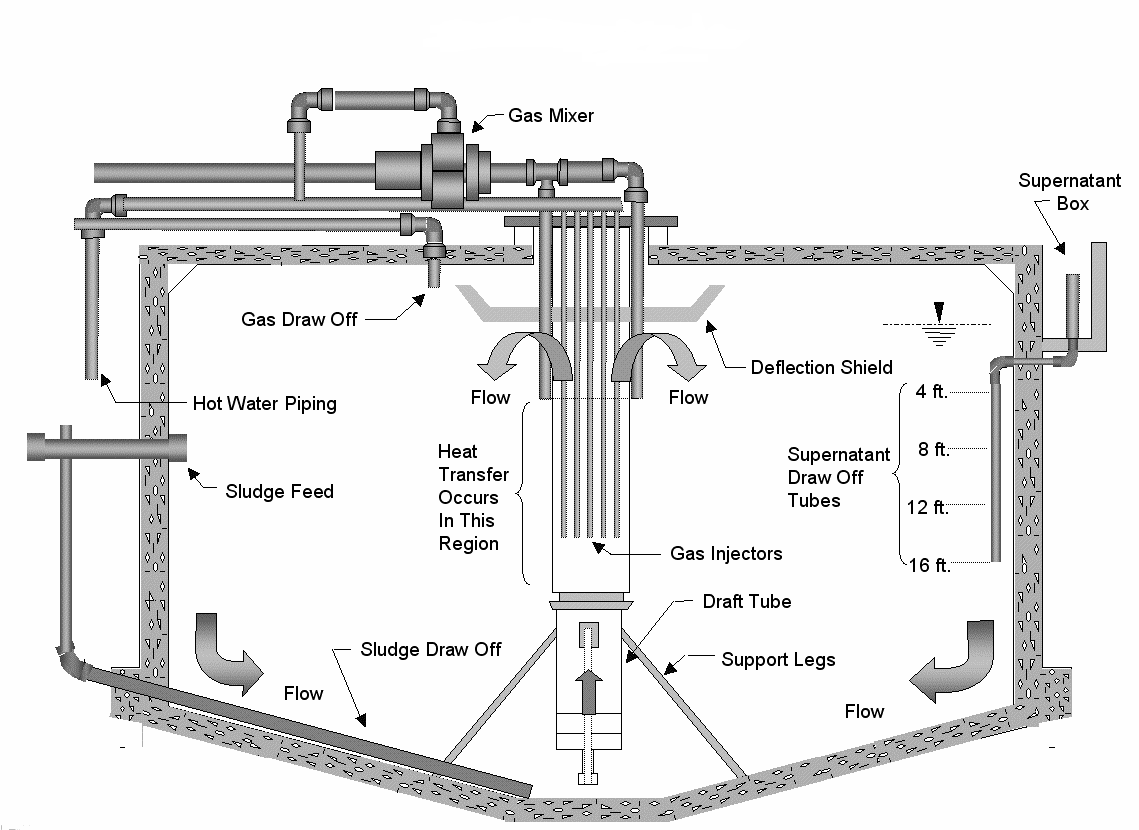
\includegraphics[scale=0.50]{DigesterFixedCover}\\
\textbf{Anaerobic Digester}\\
\end{center}
		\item The sludge typically occupies 70 - 90\% of the total digester volume and the methane carbon dioxide gas mixture occupies the headspace from where it is withdrawn also on a continuous basis.
		\item In the anaerobic digestion process microorganisms convert volatile matter into mainly methane (CH$_4$) and carbon dioxide (CO$_2$)
		\item The sludge content of the digesters is kept mixed and maintained in a constant temperature range using external heating.
		\item The activity and type of bacteria present in the digester is dictated by the operating temperature of the digester.
		\item Anaerobic digestion can be in the following three temperature ranges, each of which has its own unique microbiology.\\
			\begin{enumerate}[1. ]
			\item Psychrophilic digester:  Digester is maintained between 50  - 65 F.  Sludge detention time - 50 to 180 days
			\item Mesophilic digesters: – Digester is most commonly operated  between 95 – 98 F and the typical number of days required for digestion is between 15 to 30 days.\\
			\item Thermophilic digesters:  These digesters’ optimal operating temperatures range is between 113   135 F and it typically requires 5 to 12 days.\\
			\end{enumerate}     
		\item These organic solids are measured as volatile solids (VS).  
		\item The volatile solids content of the sludge entering and leaving the digester are measured to quantify the solids removal in the digester
		 \item Breakdown of volatile matter in the sludge ultimately into methane (CH$_4$) and carbon dioxide (CO$_2$) occurs in multiple steps involving different groups of microorganisms as follows:\\
			\begin{enumerate}[Step 1.]
			\item Hydrolysis:  Here the microorganisms breakdown complex organic matter in the sludge - carbohydrates, proteins, lignin, and lipids into simpler compounds including sugars, soluble fatty acids and amines.\\
			\item Acid Formation:  The simpler compounds formed in Step 1 are converted to organic acids by acid forming bacteria\\
			\item Methane Formation: The organic acids formed in Step 2 are converted into methane and carbon dioxide by methane forming bacteria.\\
			\end{enumerate}
		\item Gas production ranges between 10 to 16 cubic feet per pound of volatile matter destroyed and the gas production remains stable over time.
		\item Low gas production indicates problems - toxicity, temperature, volatile acid to alkalinity ratio, mixing, or feed rates.
		\end{itemize}


\section{Sludge Dewatering}\index{Sludge Dewatering}
Solids stabilized using digestion process has only a small percentage by weight of solids -less than 5\%.  It therefore becomes necessary to dewater the stabilized sludge prior to hauling off-site for final disposal.  Like thickening, the dewatering process does not treat the sludge.  It increases the solids content to between 15 to 30 percent and the higher solids content of the stabilized sludge makes it easier to handle and reduces costs associated with elements related to accomplishing the end objectives with the sludge – land application, composting, drying, incineration or landfill.\\
Dewatering involves conditioning the sludge with a polymer and subjecting it to a physical process which include:
\begin{enumerate}
\item Belt Filter Press 
\item Centrifuge
\end{enumerate}

